\begin{longtable}{|m{10cm}|m{3cm}|}
\caption{Elemente der Ereignisgesteuerten Prozesskette} \\
\hline
\label{tab:ElementeDerEreignisgesteuertenProzesskette}
\textbf{Element} & \textbf{Symbol}\\
\hline
\textbf{Funktion} 

Funktionen beschreiben T�tigkeiten, die im Verlauf des Gesch�ftsprozesses anfallen. Sie k�nnen von Mitarbeitern oder einem Informationssystem durchgef�hrt werden und ben�tigen evtl. Ressourcen, die ihnen zugewiesen werden. 

Beispiele: \textit{Auftrag anlegen}, \textit{Rechnung schreiben}, \textit{Konto abschlie�en} & 
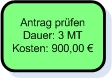
\includegraphics[width=3cm]{EPK-Funktion.jpg} \\
\hline
\textbf{Ereignis} 

Ereignisse sind betriebswirtschaftlich relevante Ereignisse, die den Gesch�ftsprozess in irgendeiner Weise steuern oder beeinflussen. Ereignisse sind immer Ausl�ser oder Ergebnisse von Funktionen. Ein Gesch�ftsprozess beginnt und endet stets mit einem Ereignis. 

Beispiele: \textit{Auftrag eingetroffen}, \textit{�berweisung get�tigt}, \textit{Rechnung erstellt} & 
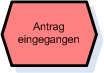
\includegraphics[width=3cm]{EPK-Ereignis.jpg} \\
\hline
\textbf{Operatoren} 

Operatoren steuern den Kontrollfluss eines Gesch�ftsprozesses. Sie machen \zB deutlich, dass eine Funktion mehrere Ereignisse ausl�st, oder zeigen alternative Vorgehensweisen an. Es gibt drei Operatoren (v.\,l.\,n.\,r.\,): UND, ODER und XODER (exklusives ODER). & 

\includegraphics[width=3cm]{EPK-Operatoren.jpg} \\
\hline
\textbf{Organisationseinheit} 

Organisationseinheiten werden Funktionen zugeordnet und beschreiben, wo die Funktionen ausgef�hrt werden bzw. wer sie ausf�hrt. Die Bezeichnung der Symbole enth�lt zus�tzlich zur Abteilung noch die Namen der Mitarbeiter.

Beispiele: \textit{Vertrieb}, \textit{Personal}, \textit{Produktion} & 
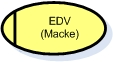
\includegraphics[width=3cm]{EPK-Organisationseinheit.jpg} \\
\hline
\textbf{Informationsobjekt} 

Auch Informationsobjekte werden Funktionen zugewiesen und beschreiben die von diesen ben�tigten oder erstellten Informationen. Dabei sind s�mtliche Formen von Informationen auf verschiedenen Datentr�gern m�glich und nicht etwa nur digitale Daten. Die Bezeichnung der Symbole enth�lt zus�tzlich das Informationssystem, aus dem die Informationen stammen.

Beispiele: \textit{Kundendatenbank}, \textit{Versicherungsantrag}, \textit{Rechnung} & 
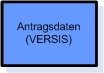
\includegraphics[width=3cm]{EPK-Informationen.jpg} \\
\hline
\textbf{Prozesswegweiser}

Mit Prozesswegweisern werden Prozesse, die in anderen EPKs beschrieben sind, referenziert. So k�nnen \zB un�bersichtliche Prozesse in Teilprozesse gegliedert und h�ufig verwendete Prozesse an zentraler Stelle modelliert werden. Prozesswegweiser stehen in einer EPK immer anstelle von Funktionen. & 
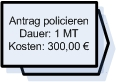
\includegraphics[width=3cm]{EPK-Prozesspfad.jpg} \\
\hline
\end{longtable}
